\subsection{Test af lavpasfilter}
For at teste om lavpasfilteret fungerer efter kravene stillet i \autoref{sec:lavpas_krav} visualiseres forskellen mellem det ufiltrede signal og det filtrede signal. Signalerne der sendes ind er fra det optagede signal fra pilotforsøget \autoref{sec:pilotforsoeg}. Disse sendes til mikrokontrollen via UART-forbindelse, hvorved der modtages den retunerede værdi. De sendte og returnerede værdier er visualiseret i MATLAB og fremgår af \autoref{fig:lavpas_imp}

\begin{figure}[H]
\centering
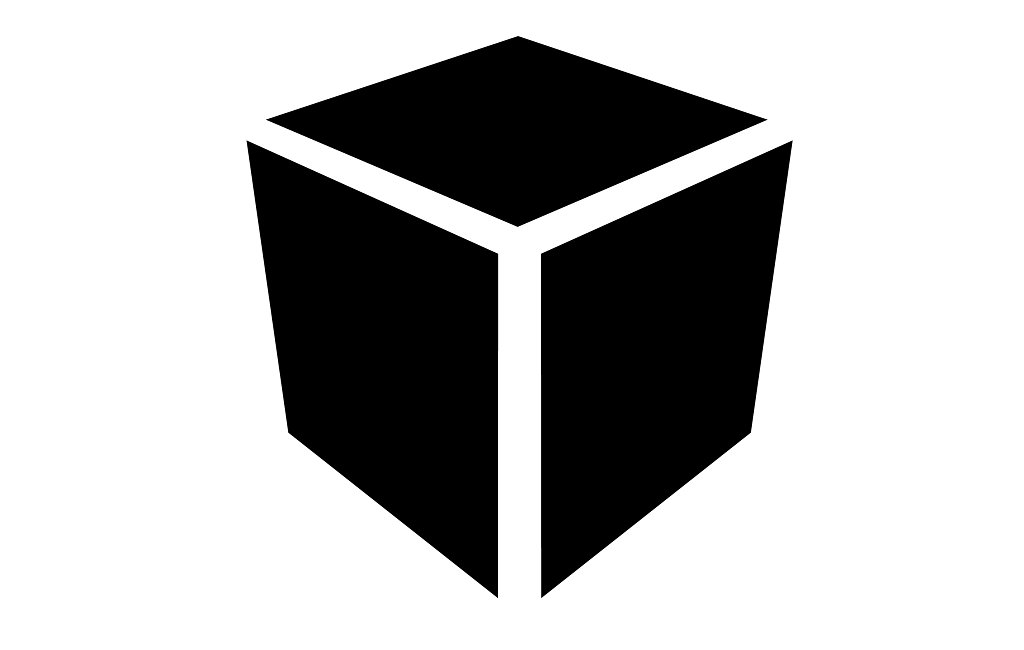
\includegraphics[width=0.8\textwidth]{figures/Pilotforsoeg/blackbox}
\caption{Lavpasfilter lavet på mikrokontrolleren visualiseret i MATLAB}
\label{fig:lavpas_imp}
\end{figure}


